\documentclass{standalone}
\usepackage{tikz}
\usetikzlibrary{arrows,calc}

\begin{document}

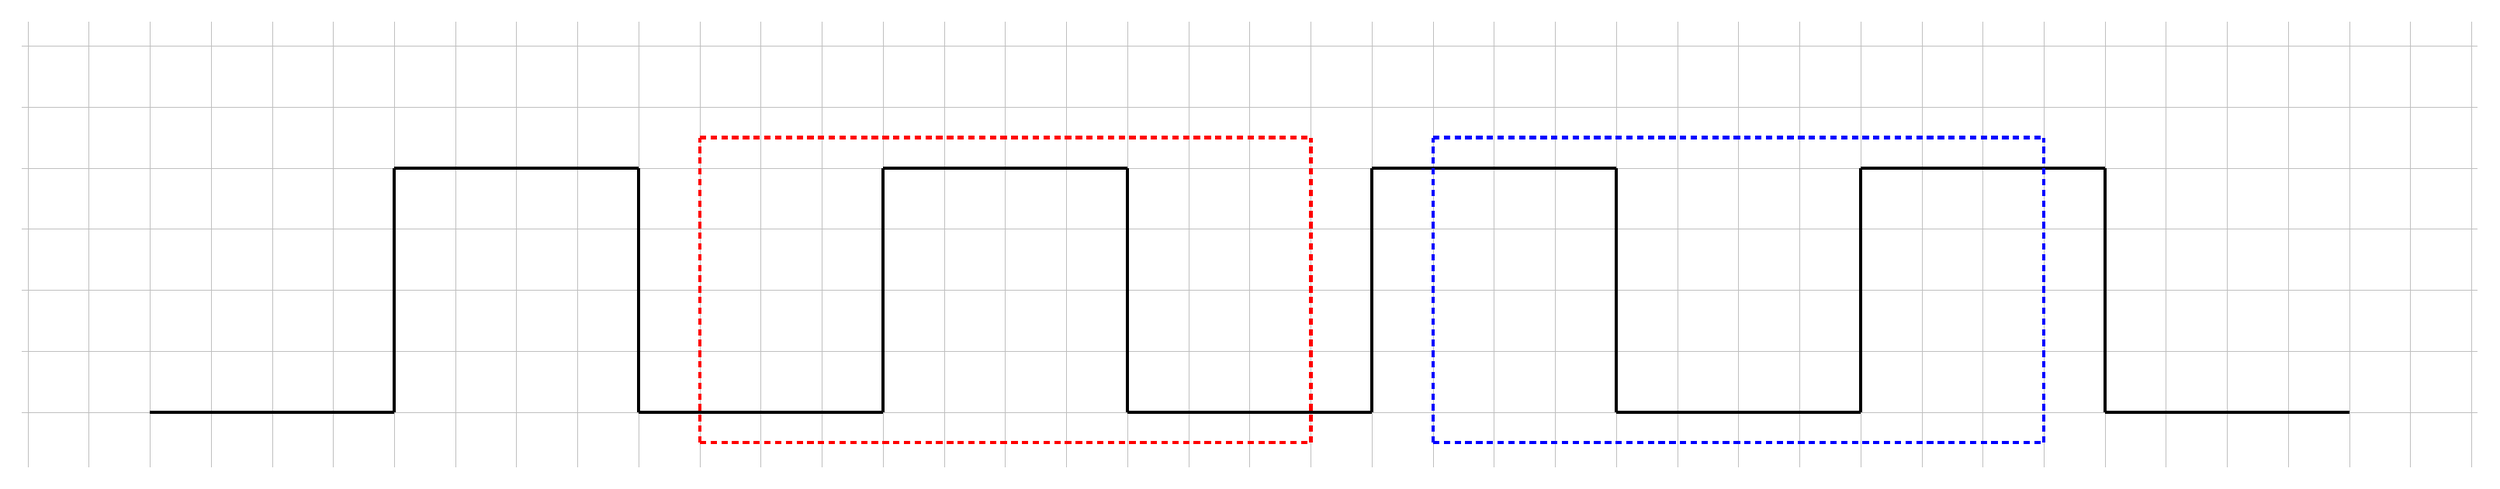
\begin{tikzpicture}
    \draw[very thin,color=gray!50] (-8.1,-0.9) grid (32.1,6.4);
%    \draw[->] (-5.2,0) -- (5.2,0) node[right] {$x$};
%    \draw[->] (0,-0.2) -- (0,5.2) node[above] {$f(x)$};
    \draw[-,ultra thick] (-2,4) -- (2,4); 
    \draw[-,ultra thick] (-2,0) -- (-2,4);
    \draw[-,ultra thick] (2,0) -- (2,4);

    \draw[-,ultra thick] (2,0) -- (6,0);
    \draw[-,ultra thick] (-2,0) -- (-6,0);

    \draw[-,ultra thick] (10,0) -- (10,4); 
    \draw[-,ultra thick] (6,0) -- (6,4);
    \draw[-,ultra thick] (6,4) -- (10,4);

    \draw[-,ultra thick] (10,0) -- (14,0);

    \draw[-,ultra thick] (14,0) -- (14,4); 
    \draw[-,ultra thick] (18,0) -- (18,4);
    \draw[-,ultra thick] (14,4) -- (18,4);

    \draw[-,ultra thick] (18,0) -- (22,0);

    \draw[-,ultra thick] (22,0) -- (22,4); 
    \draw[-,ultra thick] (26,0) -- (26,4);
    \draw[-,ultra thick] (22,4) -- (26,4);

    \draw[-,ultra thick] (26,0) -- (30,0);

% Box the window
    \draw[-,red, ultra thick, densely dashed] (3,-0.5) -- (3,4.5);
    \draw[-,red, ultra thick, densely dashed] (13,-0.5) -- (13,4.5);
    \draw[-,red, ultra thick, densely dashed] (3,-0.5) -- (13,-0.5);
    \draw[-,red, ultra thick, densely dashed] (3,4.5) -- (13,4.5);

% Box shift window

    \draw[-,blue, ultra thick, densely dashed] (15,-0.5) -- (15,4.5);
    \draw[-,blue, ultra thick, densely dashed] (25,-0.5) -- (25,4.5);
    \draw[-,blue, ultra thick, densely dashed] (15,-0.5) -- (25,-0.5);
    \draw[-,blue, ultra thick, densely dashed] (15,4.5) -- (25,4.5);

\end{tikzpicture}
\end{document} 
